\chapter{Forskningsmetoder}
\label{ch:method}
Dette kapittelet redegjør for forskningsmetodene til prosjektet. Forskningsstrategiene og datagenereringsmetodene
tar utgangspunkt i \citet{oates}. Se figur \ref{fig:oates_model} for en oversikt over forskningsrammeverket.

\begin{figure}
\centering
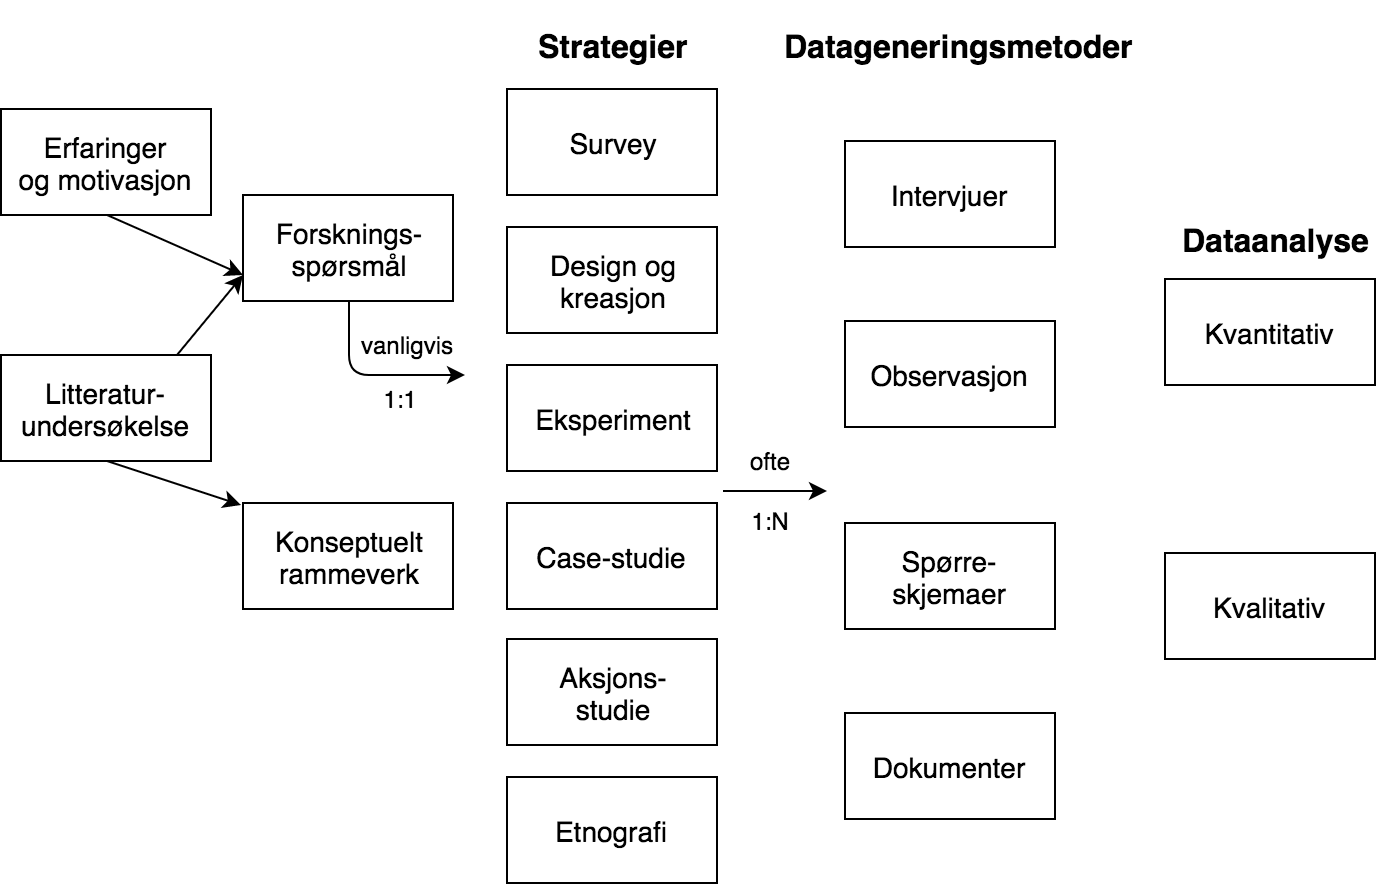
\includegraphics[width=0.95\textwidth]{fig/oates/oates_research_norwegian_final}
\caption{Modell av forskningsprosessen fra \citet{oates}.}
\label{fig:oates_model}
\end{figure}

\section{Forskningsstrategier}
En forskningsstrategi er en overordnet tilnærming for å svare på et forskningsspørsmål \citep[s. 35]{oates}.

\subsection{Design og kreasjon}
\textquote[\cite{oates}]{Forskningsmetoden design og kreasjon fokuserer på utvikling av nye IT-produkter, også kalt \textit{artefakter}.
Typer IT-artifakter inkluderer: begreper, modeller, metoder og implementasjoner}{.}
Hovedpoenget er å lære gjennom å lage, og \citet{oates} identifiserer fem steg for denne prosessen:

\begin{description}
  \item[Bevisstgjøring] Hva er problemet? Hva er rammene for problemet?
  \item[Forslag] Hvordan kan problemet løses? Hva er ideen?
  \item[Utvikling] Problemløsingsfasen. Implementasjon av løsning.
  \item[Evaluering] Hvordan gikk dette? Hva var forventningene?
  \item[Konklusjon] Hva kan vi trekke ut av dette? Hva må man se mer på?
\end{description}

I følge \citet[s.121-122]{oates} er fordelene til design og kreasjon-strategien at det er enklere å relatere til noe
som eksisterer i virkeligheten enn en íde, en tanke eller et konsept.
Den raske teknologiutviklingen gjør også at det er mulig å foreslå og utvikle nye artefakter, og at man dermed bidrar til ny kunnskap.

Ulempen med å velge denne strategien er at det er fort gjort at en kun demonstrerer
teknisk kompetanse uten at det kvalifiserer som god forskning. I tillegg til det nye produktet må ny kunnskap utvikles, bygget
på analyse, argumenter og kritiske evalueringer \citep[s. 109]{oates}. En ting er at det lages et nytt produkt i et domene --
viktigere momenter er hvilken ny informasjon den fører med seg og konteksten den blir satt inn i.

\subsection{Case-studie}
Yin (2003) definerer i følge \citet{oates} case-studie som \textquote{en empirisk undersøkelse
som utforsker et samtidsfenomen i kontekst til virkeligheten, spesielt når grensene mellom fenomenet
og konteksten ikke er helt klart}{.}
\textquote[\cite{oates}]{En case-studie fokuserer på én instans av det som skal undersøkes: en organisasjon, en avdeling, et informasjonssystem,
    et diskusjonsforum (...). Denne ene instansen, eller tilfellet, studeres i detalj med forskjellige datagenereringsmetoder som
    intervju, observasjon, dokumenter (...)}{.}

Det som kjennetegner en case-studie er at det mer fokus på dybde snarere enn bredde,
at casen undersøkes i en naturlig ramme på en helhetlig måte, med flere kilder og metoder \citep[s. 142]{oates}. En undersøkende case-studie er nyttig for å kunne forstå
forskningsområdet bedre og definere gode forskningsspørsmål,
spesielt dersom det eksisterer lite forskning allerede, mens en beskrivende studie vil rette seg mer
mot å belyse én sak fra flere sider i en helhetlig historie. Den siste typen
case-studie er forklarende, og ønsker å finne ut hvorfor noe spesielt skjedde og hva
som forårsaket det \citep[s. 143]{oates}.

Ulemper med denne strategien er, i følge \citet{oates}, at mangelen på streng krav kan føre til generaliseringer med
lav kredibilitet, at det kan være
vanskelig å få tilgang til riktige personer og riktig informasjon, samt at forskeren i seg selv kan påvirke mye av det som blir gjort fordi det er
så få regler.
    
\subsection{Prototyping}
En prototype er en implementasjon av en artefakt som ikke er produksjonsklar, eller som ikke nødvendigvis er ment for å
bli helt ferdig i fremtiden. Ved prototyping vil man ofte lage flere ulike modeller som er delvis ferdige
for å finne ut hva som egner seg, og for å få ny kunnskap om det som lages. Det er lettere å endre på noe iterativt
på prototypestadiet enn på produksjonsstadiet.

Man skiller vanligvis mellom prototyper som er lavnivå og høynivå. Lavnivå prototyper er enkle og kan lett endres.
Eksempler er for eksempel papirprototyper der knapper og bokser kan flyttes på for å endre designet og skisser.
Høynivå prototyper vil derimot ligne mer på sluttproduktet med bruk av ekte materialer, og kanskje programvare
på alfa- eller betanivå som delvis fungerer.

\subsection{Brukersentrert utvikling}
Brukersentrert utvikling er en prosess der brukeren er involvert i hvert steg.
Stegene er å forstå brukskonteksten, etablere krav, implementere artefakt og evaluere artefakt. Dette er en syklus som kan gjentas flere ganger.
\citet{dis20099241} standardiserer brukersentrert utvikling. Se figur \ref{fig:iso9241-210}
for de ulike stegene i prosessen.
Brukersentrert utvikling passer godt inn i de fem stegene som inngår i «design og kreasjon»-forskningsmetoden. Prosessen fungerer best hvis den gjentas
flere ganger, gjerne med en lavnivå prototype som gradvis nærmer seg mer og mer produksjonsklar.

\begin{figure}
\centering
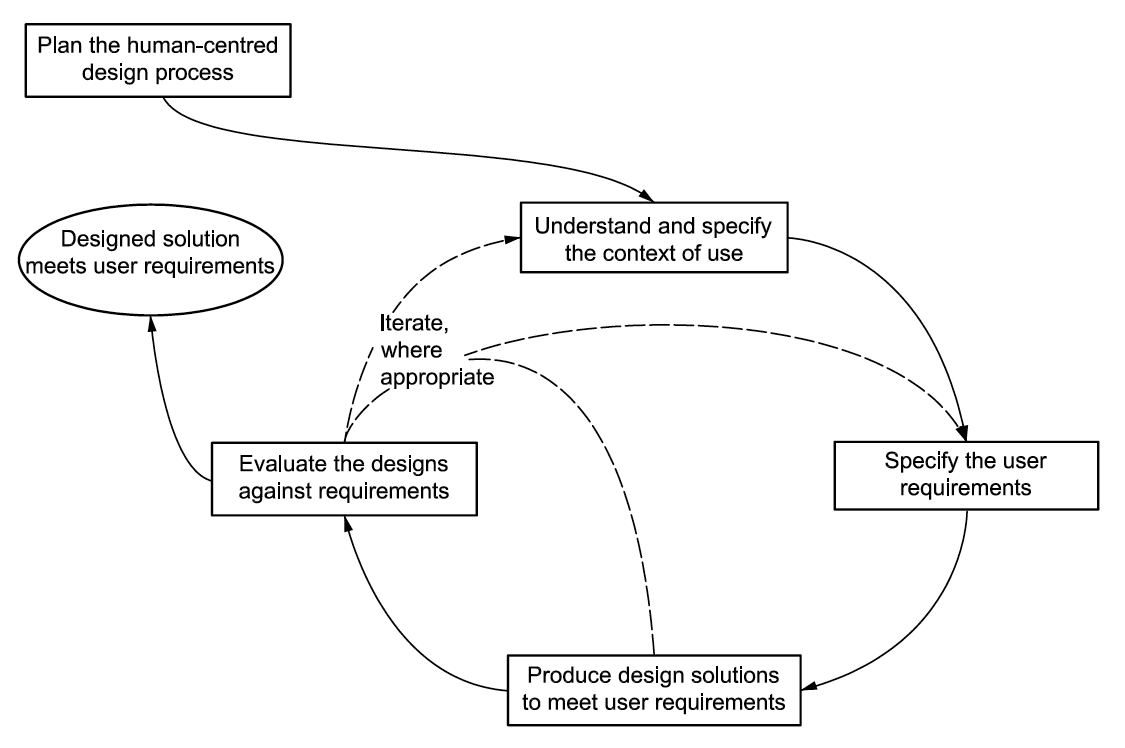
\includegraphics[width=0.85\textwidth]{fig/iso9241-210}
\caption{Gjensidige avhengigheter innenfor menneskeorientert designaktiviteter \citep{dis20099241}.}
\label{fig:iso9241-210}
\end{figure}

\section{Datagenereringsmetoder}
En datageneringsmetode er måten man innhenter empirisk materiale og data i kvalitativ
eller kvantitativ form \citep[s. 36]{oates}.

\subsection{Semistrukturert intervju}
Det finnes flere forskjellige typer intervju. Semistrukurert intervju er en datagenereringsmetode
der noen temaer og spørsmål er forberedt på forhånd, men rekkefølgen spørsmålene stilles i kan endre seg
og nye temaer og spørsmål kan komme opp basert på samtalen man har med intervjuobjektet. Det er et
kompromiss mellom et strukturert intervju og et helt ustrukturert intervju \citep[s. 188]{oates}.

Det er en mye brukt metode i case-studier for å få detaljert informasjon ut av intervjuobjektet.
I tillegg kan metoden brukes til å få tilbakemeldinger fra brukere på en kravspesifikasjon og en
endelige prototype \citep[s. 187]{oates}.

Det er vanlig at intervjuer transkriberes og analyseres som et dokument i etterkant, spesielt
hvis det er snakk om semi-eller ustrukturerte intervjuer. Her kan kildene
få mulighet til å gå over svarene i intervjuet dersom de ønsker det, siden det aldri vil være mulig
å transkribere noe helt likt det muntlige som ble sagt i samtalen.

\subsection{Dokumenter}
Dokumenter kan deles inn i to kategorier: dokumenter som eksisterer før forskningen og dokumenter laget underveis
i forskningen. Eksempler på førstnevnte er offentlig informasjon en kommune har lagt ut på Internett, rapporter
om velferdsteknologi og råd fra myndigheter. Dokumenter som lages underveis i forskningen kan for eksempel være
bilder tatt i en case-studie, transkribering av intervjuer
og modeller og diagrammer knyttet til en spesiell implementasjon av en artefakt \citep[s. 233-234]{oates}.

En bredere definisjon av dokumenter kan også med fordel benyttes. Det er ikke bare snakk om side på side med tekst på papir,
men multimediaelementer som nettsider, spill, videoer, applikasjoner og nettforum \citep[s. 235]{oates}.

Det er to ulike tilnærminger til analysering av dokumenter: dokumenter som beholder for data og dokumenter som objekter i seg selv.
Førstnevnte metode der dokumenter er entiteter som inneholder data er relevant for dette forskningsprosjektet.
Med denne metoden kan en enten for eksempel telle hvor mange ganger et ord opptrer i et dokument (kvantiativt),
eller så kan en kvalitativt analysere hvilke temaer som var til stede i dokumentet (kvalitativt) med tekstmarkering.
